\newpage
\section{Diagrammi dei packages}

\subsection{Introduzione}
Questa sezione racchiude i diagrammi dei packages, raccolti tramite un approccio top-down. Considerando l'approccio adottato e il particolare applicativo realizzato con un pattern a Microservizi, non ci discosteremo dalla nomenclatura tradizionale di \textit{Classe} intesa come una categoria di entità in grado di svolgere uno specifico compito. Per mantenere una conformità con lo standard UML\ped{G} dunque, verrà utilizzato il termine \textit{classe} per indicare ciò che all'atto pratico sarà implementato come un microservizio vero e proprio, stand-alone, e con i propri metodi in grado di fornire la funzionalità preposta. Trattandosi di una progettazione con un livello di dettaglio intermedio, le classi non verranno definite, bensì verrà data una descrizione della loro funzionalità, lo scopo e le relazioni che intercorrono con le altre classi.

L'applicativo API Market è strutturato, come di consueto, in un lato Front-end ed un lato Back-end, come mostrato dal diagramma seguente:

\begin{figure}[H]
	\centering
	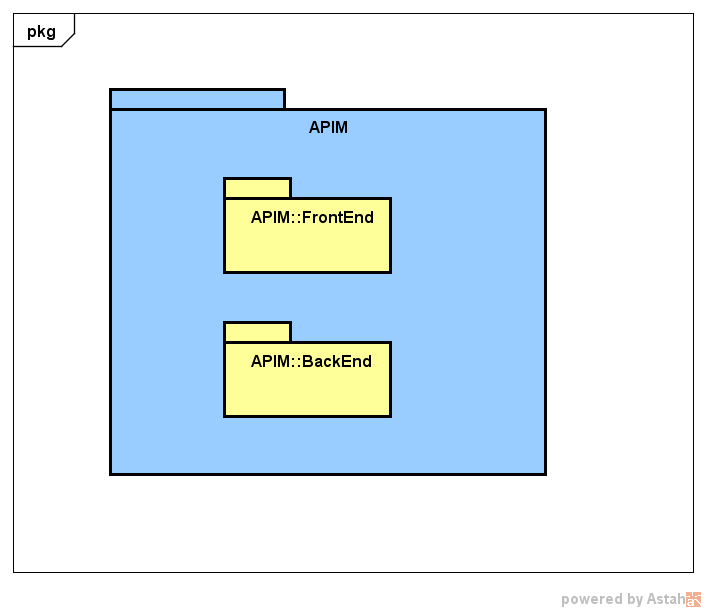
\includegraphics
	[width=0.7\linewidth]
	{UML/DiagrammiPackage/APIM.png}
	\caption{Package APIM}
\end{figure}

\subsection{Front-end}

Il lato front-end risulta così strutturato:

\begin{figure}[H]
	\centering
	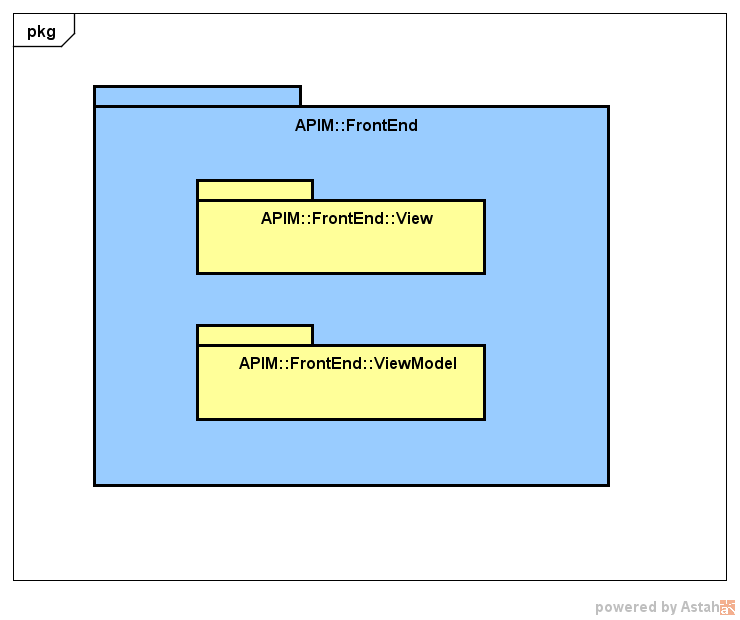
\includegraphics
	[width=0.7\linewidth]
	{UML/DiagrammiPackage/FrontEnd.png}
	\caption{Package APIM::FrontEnd}
\end{figure}

Nella parte front-end sono dunque presenti i package View e ViewModel che rispecchiano l'architettura nativa dei framework da noi utilizzati.

\subsubsection{View}

Il package per il componente View contiene i seguenti sub-packages:

\begin{figure}[H]
	\centering
	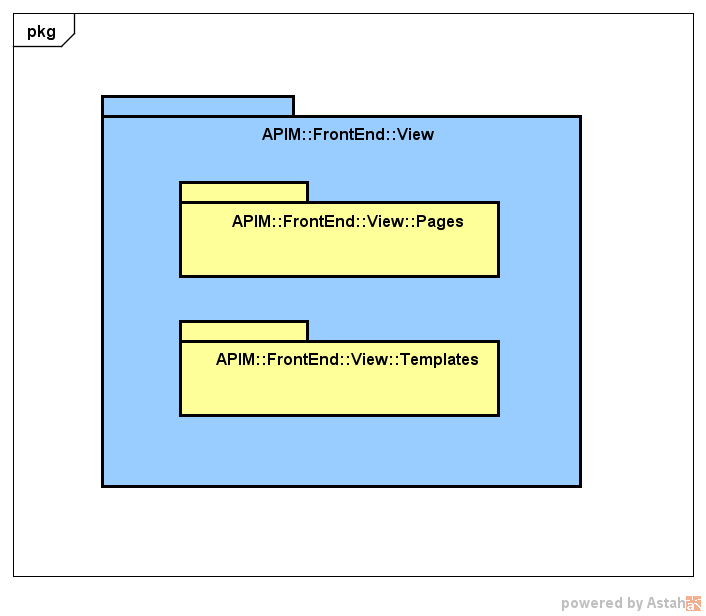
\includegraphics
	[width=0.7\linewidth]
	{UML/DiagrammiPackage/View.png}
	\caption{Package APIM::FrontEnd::View}
\end{figure}

\begin{itemize}
	\item \textbf{Pages}: Il package \textit{Pages} contiene una classe astratta \textit{Page}. Essa è poi utilizzabile tramite una derivazione concreta di tale classe, e l'implementazione avviene a seconda di ciò che è necessario visualizzare. Tali implementazioni possono usufruire dei template, per gestire situazioni standardizzate.
	\item \textbf{Templates}: Il package \textit{Templates} contiene un modello standard delle componenti utilizzabili per la rappresentazione. Ogni pagina che presenta situazioni e modelli analoghi può utilizzare un template già definito, per un maggior riuso, e per distinguere nettamente gli elementi contenuti in una pagina dalla loro realizzazione.
\end{itemize}


\paragraph{Pages}

\begin{figure}[H]
	\centering
	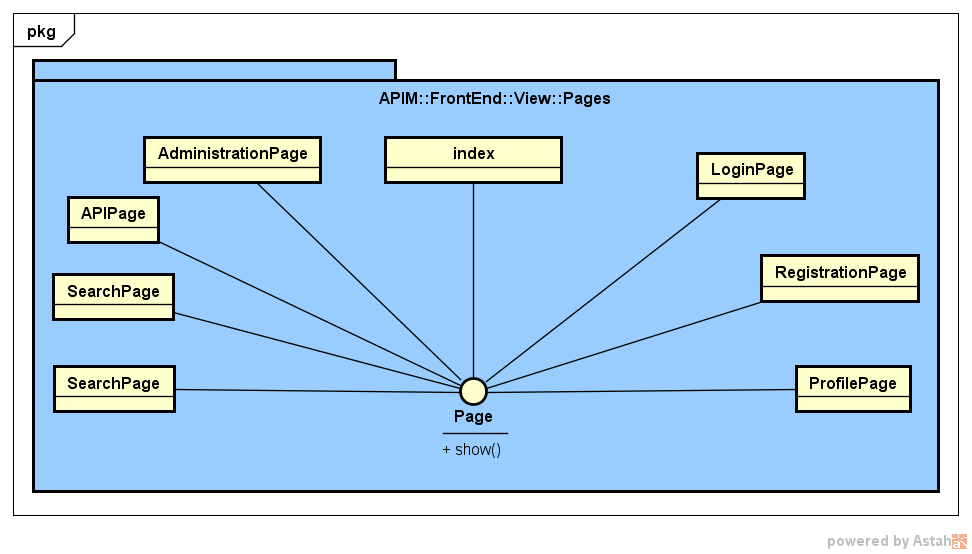
\includegraphics
	[width=0.7\linewidth]
	{UML/DiagrammiPackage/Pages.png}
	\caption{Package APIM::FrontEnd::View::Pages}
\end{figure}

\subparagraph{Page}
\begin{itemize}
	\item \textbf{Funzione del componente}: rappresenta una pagina web.
	\item \textbf{Relazioni d’uso di altri componenti}: interfaccia di base da cui derivano le altre pagine web.
	\item \textbf{Attività svolte e dati trattati}: definisce le caratteristiche minime che ogni pagina deve possedere.
\end{itemize}

\subparagraph{Index}
\begin{itemize}
	\item \textbf{Funzione del componente}: rappresenta la pagina principale dell'API Market.
	\item \textbf{Relazioni d’uso di altri componenti}: concretizza l'interfaccia Page e utilizza i template MainMenu e SearchForm.
	\item \textbf{Attività svolte e dati trattati}: permette l'autentificazione dell'utente.
\end{itemize}

\subparagraph{LoginPage}
\begin{itemize}
	\item \textbf{Funzione del componente}: rappresenta la pagina di login.
	\item \textbf{Relazioni d’uso di altri componenti}: concretizza l'interfaccia Page e utilizza il template LoginForm.
	\item \textbf{Attività svolte e dati trattati}: permette l'autentificazione dell'utente.	
\end{itemize}

\subparagraph{RegistrationPage}
\begin{itemize}
	\item \textbf{Funzione del componente}: 
	\item \textbf{Relazioni d’uso di altri componenti}: 
	\item \textbf{Attività svolte e dati trattati}: 	
\end{itemize}

\subparagraph{ProfilePage}
\begin{itemize}
	\item \textbf{Funzione del componente}: 
	\item \textbf{Relazioni d’uso di altri componenti}: 
	\item \textbf{Attività svolte e dati trattati}: 	
\end{itemize}

\subparagraph{AdministrationPage}
\begin{itemize}
	\item \textbf{Funzione del componente}: 
	\item \textbf{Relazioni d’uso di altri componenti}: 
	\item \textbf{Attività svolte e dati trattati}: 	
\end{itemize}

\subparagraph{APIPage}
\begin{itemize}
	\item \textbf{Funzione del componente}: 
	\item \textbf{Relazioni d’uso di altri componenti}: 
	\item \textbf{Attività svolte e dati trattati}: 	
\end{itemize}

\subparagraph{SearchPage}
\begin{itemize}
	\item \textbf{Funzione del componente}: 
	\item \textbf{Relazioni d’uso di altri componenti}: 
	\item \textbf{Attività svolte e dati trattati}: 	
\end{itemize}

\subparagraph{CategoryListPage}
\begin{itemize}
	\item \textbf{Funzione del componente}: 
	\item \textbf{Relazioni d’uso di altri componenti}: 
	\item \textbf{Attività svolte e dati trattati}: 	
\end{itemize}


\paragraph{Templates}

\begin{figure}[H]
	\centering
	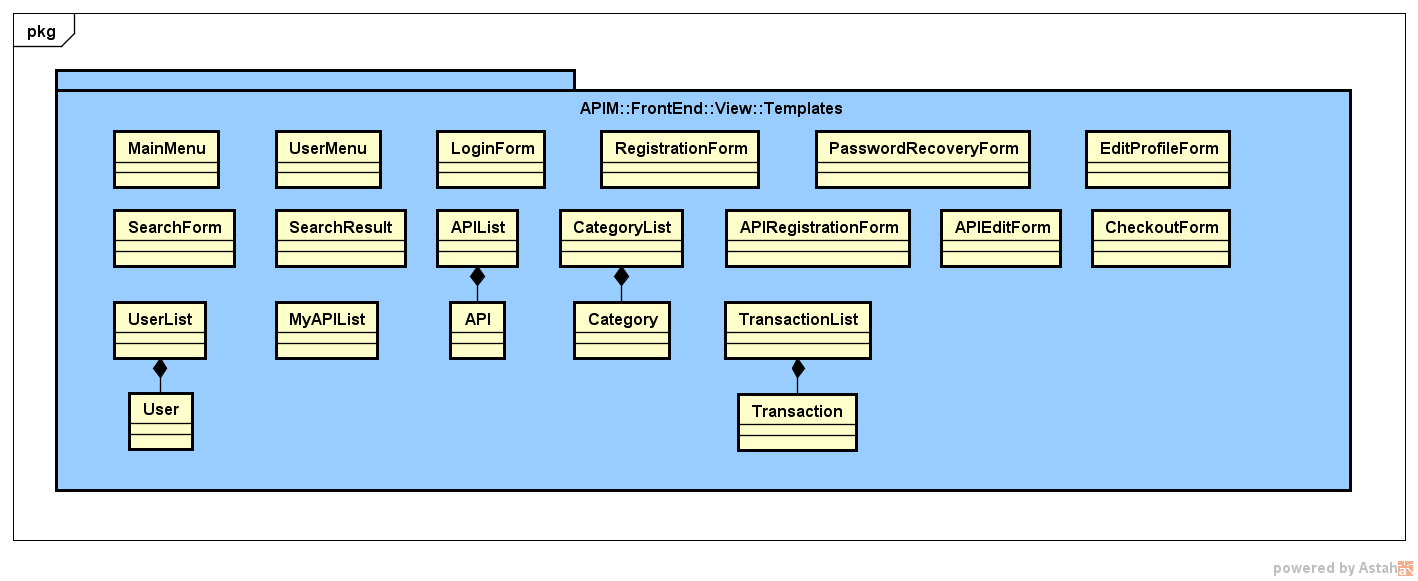
\includegraphics
	[width=0.7\linewidth]
	{UML/DiagrammiPackage/Templates.png}
	\caption{Package APIM::FrontEnd::View::Templates}
\end{figure}

\subparagraph{MainMnu}
\begin{itemize}
	\item \textbf{Funzione del componente}: 
	\item \textbf{Relazioni d’uso di altri componenti}: 
	\item \textbf{Attività svolte e dati trattati}: 
\end{itemize}

\subparagraph{UserMenu}
\begin{itemize}
	\item \textbf{Funzione del componente}: 
	\item \textbf{Relazioni d’uso di altri componenti}: 
	\item \textbf{Attività svolte e dati trattati}: 
\end{itemize}

\subparagraph{LoginForm}
\begin{itemize}
	\item \textbf{Funzione del componente}: 
	\item \textbf{Relazioni d’uso di altri componenti}: 
	\item \textbf{Attività svolte e dati trattati}: 
\end{itemize}

\subparagraph{RegistrationForm}
\begin{itemize}
	\item \textbf{Funzione del componente}: 
	\item \textbf{Relazioni d’uso di altri componenti}: 
	\item \textbf{Attività svolte e dati trattati}: 
\end{itemize}

\subparagraph{PasswordRecoveryForm}
\begin{itemize}
	\item \textbf{Funzione del componente}: 
	\item \textbf{Relazioni d’uso di altri componenti}: 
	\item \textbf{Attività svolte e dati trattati}: 
\end{itemize}

\subparagraph{EditPorfileForm}
\begin{itemize}
	\item \textbf{Funzione del componente}: 
	\item \textbf{Relazioni d’uso di altri componenti}: 
	\item \textbf{Attività svolte e dati trattati}: 
\end{itemize}

\subparagraph{SearchForm}
\begin{itemize}
	\item \textbf{Funzione del componente}: 
	\item \textbf{Relazioni d’uso di altri componenti}: 
	\item \textbf{Attività svolte e dati trattati}: 
\end{itemize}

\subparagraph{SearchResultForm}
\begin{itemize}
	\item \textbf{Funzione del componente}: 
	\item \textbf{Relazioni d’uso di altri componenti}: 
	\item \textbf{Attività svolte e dati trattati}: 
\end{itemize}

\subparagraph{API}
\begin{itemize}
	\item \textbf{Funzione del componente}: 
	\item \textbf{Relazioni d’uso di altri componenti}: 
	\item \textbf{Attività svolte e dati trattati}: 
\end{itemize}

\subparagraph{APIList}
\begin{itemize}
	\item \textbf{Funzione del componente}: 
	\item \textbf{Relazioni d’uso di altri componenti}: 
	\item \textbf{Attività svolte e dati trattati}: 
\end{itemize}

\subparagraph{Category}
\begin{itemize}
	\item \textbf{Funzione del componente}: 
	\item \textbf{Relazioni d’uso di altri componenti}: 
	\item \textbf{Attività svolte e dati trattati}: 
\end{itemize}

\subparagraph{CategoryList}
\begin{itemize}
	\item \textbf{Funzione del componente}: 
	\item \textbf{Relazioni d’uso di altri componenti}: 
	\item \textbf{Attività svolte e dati trattati}: 
\end{itemize}

\subparagraph{APIRegistrationForm}
\begin{itemize}
	\item \textbf{Funzione del componente}: 
	\item \textbf{Relazioni d’uso di altri componenti}: 
	\item \textbf{Attività svolte e dati trattati}: 
\end{itemize}

\subparagraph{APIEditForm}
\begin{itemize}
	\item \textbf{Funzione del componente}: 
	\item \textbf{Relazioni d’uso di altri componenti}: 
	\item \textbf{Attività svolte e dati trattati}: 
\end{itemize}

\subparagraph{CheckoutForm}
\begin{itemize}
	\item \textbf{Funzione del componente}: 
	\item \textbf{Relazioni d’uso di altri componenti}: 
	\item \textbf{Attività svolte e dati trattati}: 
\end{itemize}

\subparagraph{User}
\begin{itemize}
	\item \textbf{Funzione del componente}: 
	\item \textbf{Relazioni d’uso di altri componenti}: 
	\item \textbf{Attività svolte e dati trattati}: 
\end{itemize}

\subparagraph{UserList}
\begin{itemize}
	\item \textbf{Funzione del componente}: 
	\item \textbf{Relazioni d’uso di altri componenti}: 
	\item \textbf{Attività svolte e dati trattati}: 
\end{itemize}

\subparagraph{MyAPIList}
\begin{itemize}
	\item \textbf{Funzione del componente}: 
	\item \textbf{Relazioni d’uso di altri componenti}: 
	\item \textbf{Attività svolte e dati trattati}: 
\end{itemize}

\subparagraph{Transaction}
\begin{itemize}
	\item \textbf{Funzione del componente}: 
	\item \textbf{Relazioni d’uso di altri componenti}: 
	\item \textbf{Attività svolte e dati trattati}: 
\end{itemize}

\subparagraph{TransactionList}
\begin{itemize}
	\item \textbf{Funzione del componente}: 
	\item \textbf{Relazioni d’uso di altri componenti}: 
	\item \textbf{Attività svolte e dati trattati}: 
\end{itemize}


\subsubsection{ViewModel}

Il package per il componente ViewModel contiene i seguenti sub-packages:

\begin{figure}[H]
	\centering
	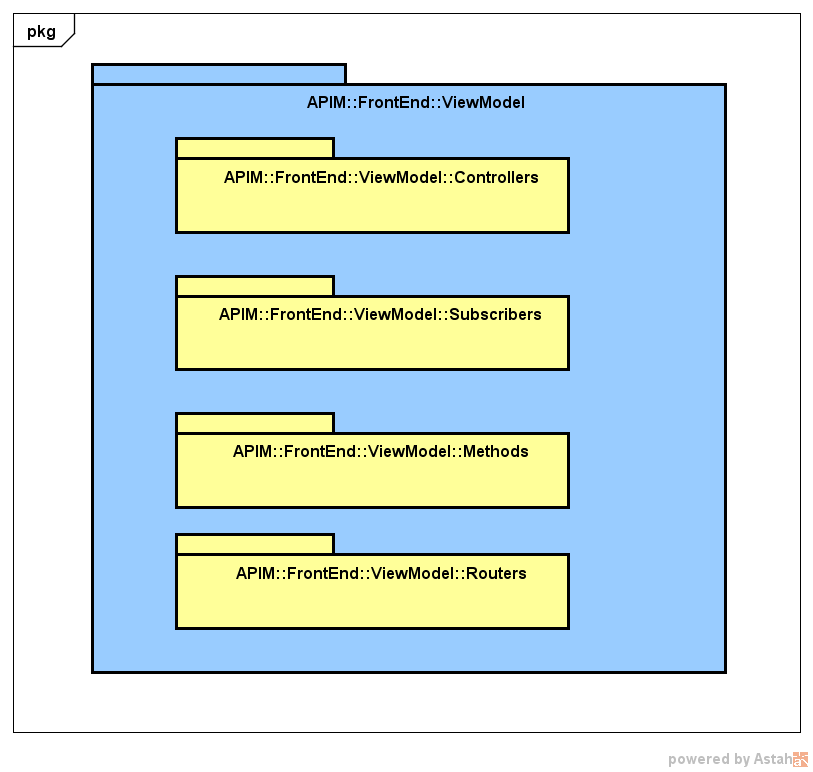
\includegraphics
	[width=0.7\linewidth]
	{UML/DiagrammiPackage/ViewModel.png}
	\caption{Package APIM::FrontEnd::ViewModel}
\end{figure}

La componente \textit{ViewModel} ha il compito di realizzare il data-binding con i componenti della \textit{View}, interagendo con la componente \textit{Model} che fornisce i dati o ne permette la modifica. La componente \textit{Model} è parte del lato back-end della piattaforma, sebbene adottando un tale approccio si ha una linea di demarcazione meno netta tra le due parti. Di seguito si analizzano i packages contenuti all'interno del componente \textit{ViewModel}

\begin{itemize}
	\item \textbf{Controllers}: contiene i controller necessari alle views per comunicare con il model. 
	\item \textbf{Subscribers}: contiene le classi necessarie al subscribing alle collezioni pubblicate dai Publisher.  
	\item \textbf{Methods}: contiene le classi necessarie a Meteor per la corretta fruizione dei dati.
	\item \textbf{Routers}: contiene la classe che esegue il routing dell'intera applicazione. 
\end{itemize}


\paragraph{Controllers}

\begin{figure}[H]
	\centering
	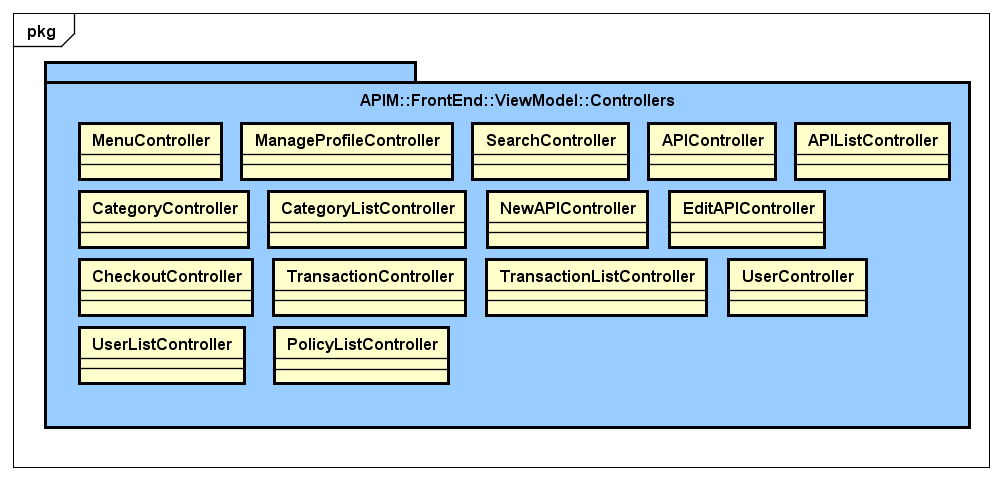
\includegraphics
	[width=0.7\linewidth]
	{UML/DiagrammiPackage/Controllers.png}
	\caption{Package APIM::FrontEnd::ViewModel::Controllers}
\end{figure}

\subparagraph{MenuController}
\begin{itemize}
	\item \textbf{Funzione del componente}: la classe permette la corretta visualizzazione del menu in base ai propri privilegi.
	\item \textbf{Relazioni d’uso di altri componenti}: il controller è collegato al template MainMenu e UserMenu.
\end{itemize}

\subparagraph{ManageProfileController}
\begin{itemize}
	\item \textbf{Funzione del componente}: permette la gestione del proprio profilo utente.
	\item \textbf{Relazioni d’uso di altri componenti}: utilizza i templates ...
	\item \textbf{Attività svolte e dati trattati}: coordina tutte le funzionalità di gestione che può svolgere un utente registrato, come gestire le proprie transazioni e vedere lo stato dei suoi abbonamenti. 
\end{itemize}

\subparagraph{SearchController}
\begin{itemize}
	\item \textbf{Funzione del componente}: 
	\item \textbf{Relazioni d’uso di altri componenti}: 
	\item \textbf{Attività svolte e dati trattati}: 
\end{itemize}

\subparagraph{APIController}
\begin{itemize}
	\item \textbf{Funzione del componente}: 
	\item \textbf{Relazioni d’uso di altri componenti}: 
	\item \textbf{Attività svolte e dati trattati}: 
\end{itemize}

\subparagraph{APIListController}
\begin{itemize}
	\item \textbf{Funzione del componente}: 
	\item \textbf{Relazioni d’uso di altri componenti}: 
	\item \textbf{Attività svolte e dati trattati}: 
\end{itemize}

\subparagraph{CategoryController}
\begin{itemize}
	\item \textbf{Funzione del componente}: 
	\item \textbf{Relazioni d’uso di altri componenti}: 
	\item \textbf{Attività svolte e dati trattati}: 
\end{itemize}

\subparagraph{CategoryListController}
\begin{itemize}
	\item \textbf{Funzione del componente}: 
	\item \textbf{Relazioni d’uso di altri componenti}: 
	\item \textbf{Attività svolte e dati trattati}: 
\end{itemize}

\subparagraph{NewAPIController}
\begin{itemize}
	\item \textbf{Funzione del componente}: 
	\item \textbf{Relazioni d’uso di altri componenti}: 
	\item \textbf{Attività svolte e dati trattati}: 
\end{itemize}

\subparagraph{EditAPIController}
\begin{itemize}
	\item \textbf{Funzione del componente}: 
	\item \textbf{Relazioni d’uso di altri componenti}: 
	\item \textbf{Attività svolte e dati trattati}: 
\end{itemize}

\subparagraph{CheckoutController}
\begin{itemize}
	\item \textbf{Funzione del componente}: 
	\item \textbf{Relazioni d’uso di altri componenti}: 
	\item \textbf{Attività svolte e dati trattati}: 
\end{itemize}

\subparagraph{TransactionController}
\begin{itemize}
	\item \textbf{Funzione del componente}: 
	\item \textbf{Relazioni d’uso di altri componenti}: 
	\item \textbf{Attività svolte e dati trattati}: 
\end{itemize}

\subparagraph{TransactionListController}
\begin{itemize}
	\item \textbf{Funzione del componente}: 
	\item \textbf{Relazioni d’uso di altri componenti}: 
	\item \textbf{Attività svolte e dati trattati}: 
\end{itemize}

\subparagraph{UserController}
\begin{itemize}
	\item \textbf{Funzione del componente}: 
	\item \textbf{Relazioni d’uso di altri componenti}: 
	\item \textbf{Attività svolte e dati trattati}: 
\end{itemize}

\subparagraph{UserListController}
\begin{itemize}
	\item \textbf{Funzione del componente}: 
	\item \textbf{Relazioni d’uso di altri componenti}: 
	\item \textbf{Attività svolte e dati trattati}: 
\end{itemize}

\subparagraph{NewPolicyController}
\begin{itemize}
	\item \textbf{Funzione del componente}: 
	\item \textbf{Relazioni d’uso di altri componenti}: 
	\item \textbf{Attività svolte e dati trattati}: 
\end{itemize}

\subparagraph{EditPolicyController}
\begin{itemize}
	\item \textbf{Funzione del componente}: 
	\item \textbf{Relazioni d’uso di altri componenti}: 
	\item \textbf{Attività svolte e dati trattati}: 
\end{itemize}

\subparagraph{PolicyListController}
\begin{itemize}
	\item \textbf{Funzione del componente}: 
	\item \textbf{Relazioni d’uso di altri componenti}: 
	\item \textbf{Attività svolte e dati trattati}: 
\end{itemize}


\paragraph{Subscribers}

\begin{figure}[H]
	\centering
	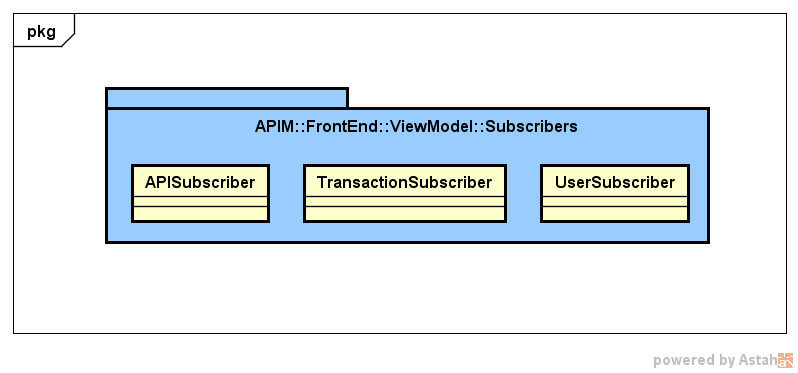
\includegraphics
	[width=0.7\linewidth]
	{UML/DiagrammiPackage/Subscribers.png}
	\caption{Package APIM::FrontEnd::ViewModel::Subscribers}
\end{figure}

\subparagraph{APISubscriber}
\begin{itemize}
	\item \textbf{Funzione del componente}: la classe esegue il subscribing delle API.
	\item \textbf{Relazioni d’uso di altri componenti}: è in relazione con l'APIController.
	\item \textbf{Attività svolte e dati trattati}: esegue il subscribing di quelle collezioni di cui è stato precedentemente fatto il publishing.
\end{itemize}

\subparagraph{TransactionSubscriber}
\begin{itemize}
	\item \textbf{Funzione del componente}: la classe esegue il subscribing delle transazioni.
	\item \textbf{Relazioni d’uso di altri componenti}: è in relazione con il TransactionController.
	\item \textbf{Attività svolte e dati trattati}: esegue il subscribing di quelle collezioni di cui è stato precedentemente fatto il publishing.
\end{itemize}

\subparagraph{UserSubscriber}
\begin{itemize}
	\item \textbf{Funzione del componente}: la classe esegue il subscribing degli utenti.
	\item \textbf{Relazioni d’uso di altri componenti}: è in relazione con lo UserController.
	\item \textbf{Attività svolte e dati trattati}: esegue il subscribing di quelle collezioni di cui è stato precedentemente fatto il publishing.
\end{itemize}

\paragraph{Methods}

\begin{figure}[H]
	\centering
	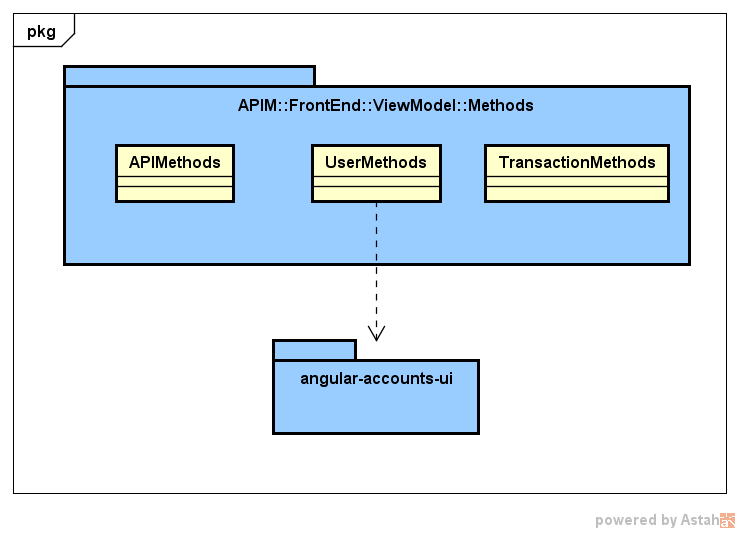
\includegraphics
	[width=0.7\linewidth]
	{UML/DiagrammiPackage/Methods.png}
	\caption{Package APIM::FrontEnd::ViewModel::Methods}
\end{figure}

\subparagraph{APIMethods}
\begin{itemize}
	\item \textbf{Funzione del componente}: la classe viene utilizzata dal Frontend per richiedere una modifica delle API.
	\item \textbf{Relazioni d’uso di altri componenti}: è in relazione con NewAPIController e EditAPIController.
	\item \textbf{Attività svolte e dati trattati}: fornisce all'utente le funzioni di inserimento, modifica e cancellazione delle API.
\end{itemize}

\subparagraph{TransactionMethods}
\begin{itemize}
	\item \textbf{Funzione del componente}: la classe viene utilizzata dal Frontend per richiedere una modifica delle transazioni.
	\item \textbf{Relazioni d’uso di altri componenti}: è in relazione con NewTransactionController e EditTransactionController.
	\item \textbf{Attività svolte e dati trattati}: fornisce all'utente le funzioni di inserimento, modifica e cancellazione delle transazioni.
\end{itemize}

\subparagraph{UserMethods}
\begin{itemize}
	\item \textbf{Funzione del componente}: la classe viene utilizzata dal Frontend per richiedere una modifica degli utenti.
	\item \textbf{Relazioni d’uso di altri componenti}: è in relazione con il package esterno angular-accounts-ui.
	\item \textbf{Attività svolte e dati trattati}: fornisce all'utente le funzioni di inserimento, modifica e cancellazione degli utenti.
\end{itemize}


\paragraph{Routers}

\begin{figure}[H]
	\centering
	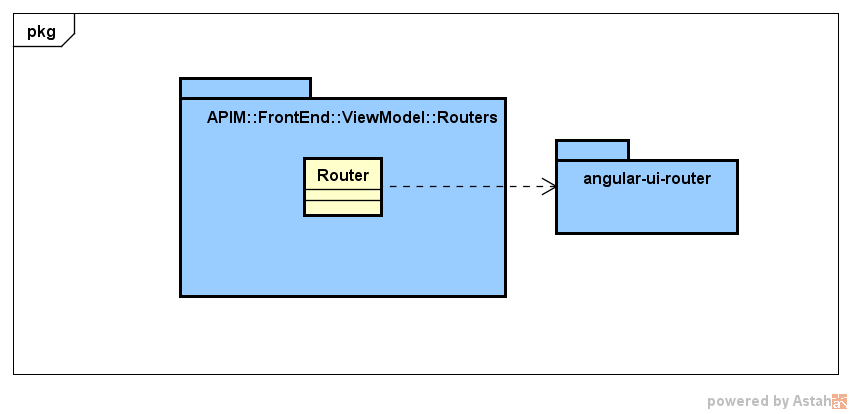
\includegraphics
	[width=0.7\linewidth]
	{UML/DiagrammiPackage/Routers.png}
	\caption{Package APIM::FrontEnd::ViewModel::Routers}
\end{figure}

\subparagraph{Router}
\begin{itemize}
	\item \textbf{Funzione del componente}: la classe permette il routing dinamico delle pagine.
	\item \textbf{Relazioni d’uso di altri componenti}: è in relazione con il package esterno angular-ui-router e con tutte le pages e i templates.
	\item \textbf{Attività svolte e dati trattati}: esegue la traduzione degli URL in modo dinamico, permettendo la visualizzazione in modalità one-page, senza bisogno di ricaricare l'intera pagina.
\end{itemize}